\section{Geom\-PQP2DRigid  Class Reference}
\label{class_GeomPQP2DRigid}\index{GeomPQP2DRigid@{Geom\-PQP2DRigid}}
2D rigid body. 


{\tt \#include $<$geom\-PQP.h$>$}

Inheritance diagram for Geom\-PQP2DRigid::\begin{figure}[H]
\begin{center}
\leavevmode
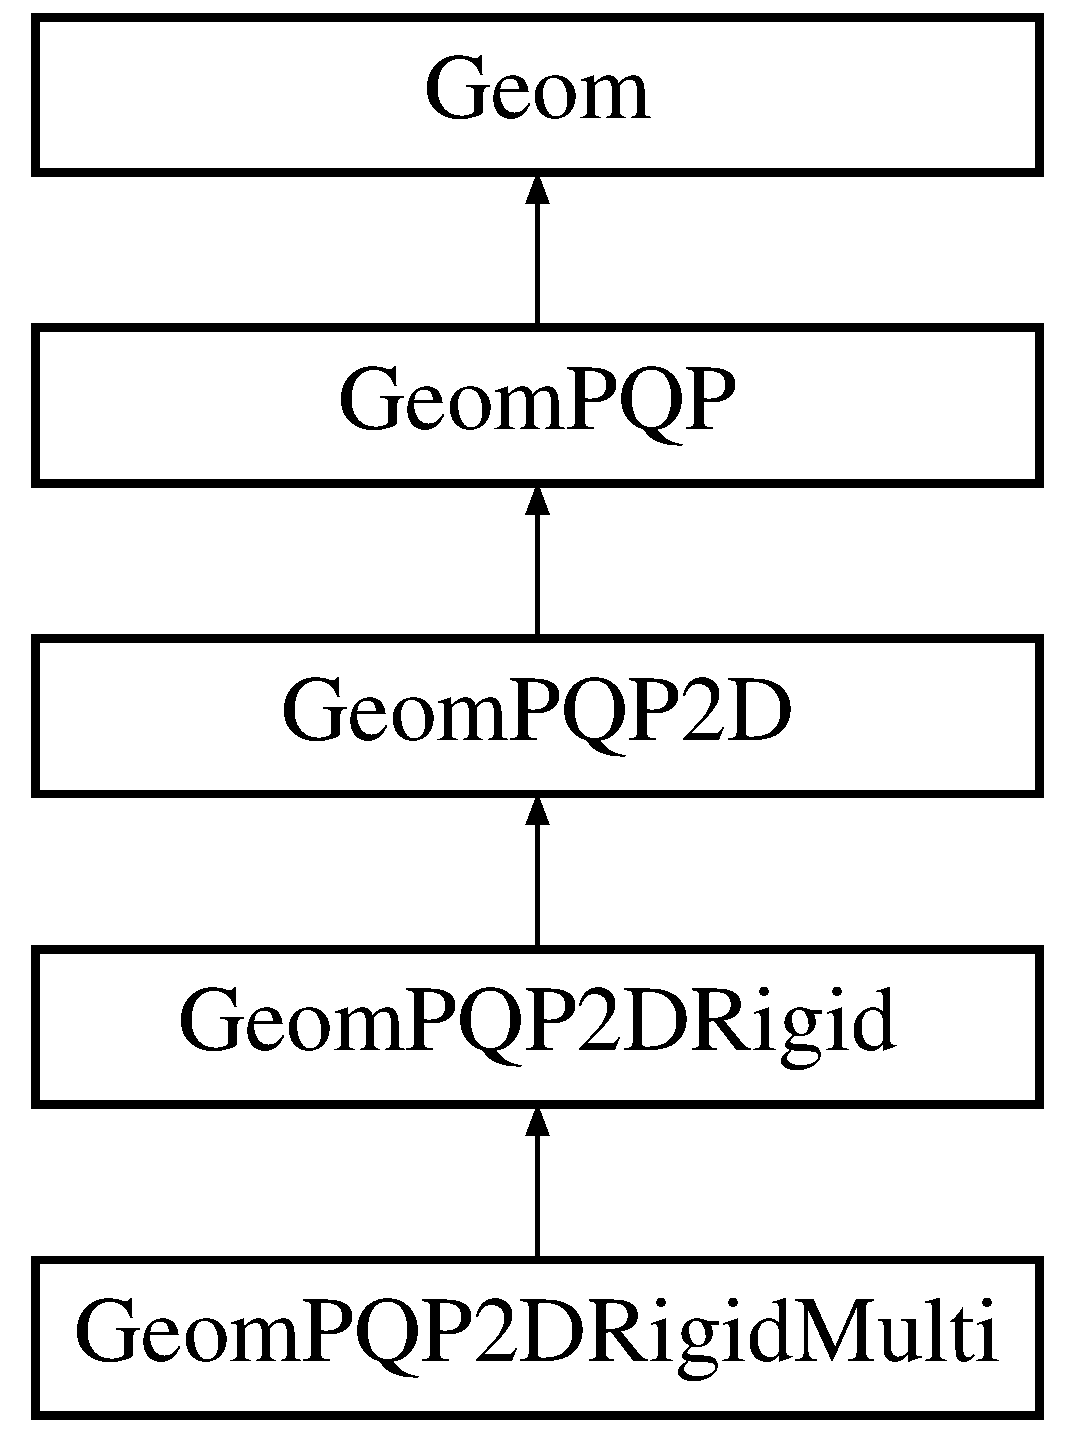
\includegraphics[height=5cm]{class_GeomPQP2DRigid}
\end{center}
\end{figure}
\subsection*{Public Methods}
\begin{CompactItemize}
\item 
{\bf Geom\-PQP2DRigid} (string path)
\item 
virtual {\bf $\sim$Geom\-PQP2DRigid} ()
\item 
virtual bool {\bf Collision\-Free} (const {\bf MSLVector} \&q)
\begin{CompactList}\small\item\em Return true if the robot(s) and obstacles are not in collision.\item\end{CompactList}\item 
virtual double {\bf Distance\-Comp} (const {\bf MSLVector} \&q)
\begin{CompactList}\small\item\em Compute the distance of the closest point on the robot to the obstacle region.\item\end{CompactList}\item 
virtual {\bf MSLVector} {\bf Configuration\-Difference} (const {\bf MSLVector} \&q1, const {\bf MSLVector} \&q2)
\begin{CompactList}\small\item\em Compute a {\bf MSLVector} {\rm (p.\,\pageref{class_MSLVector})} based on q2-q1. In R$^\wedge$n, the configurations are simply subtracted to make the {\bf MSLVector} {\rm (p.\,\pageref{class_MSLVector})}. This method exists to make things work correctly for other configuration-space topologies.\item\end{CompactList}\item 
void {\bf Set\-Transformation} (const {\bf MSLVector} \&q)
\end{CompactItemize}


\subsection{Detailed Description}
2D rigid body.



\subsection{Constructor \& Destructor Documentation}
\index{GeomPQP2DRigid@{Geom\-PQP2DRigid}!GeomPQP2DRigid@{GeomPQP2DRigid}}
\index{GeomPQP2DRigid@{GeomPQP2DRigid}!GeomPQP2DRigid@{Geom\-PQP2DRigid}}
\subsubsection{\setlength{\rightskip}{0pt plus 5cm}Geom\-PQP2DRigid::Geom\-PQP2DRigid (string {\em path})}\label{class_GeomPQP2DRigid_a0}


\index{GeomPQP2DRigid@{Geom\-PQP2DRigid}!~GeomPQP2DRigid@{$\sim$GeomPQP2DRigid}}
\index{~GeomPQP2DRigid@{$\sim$GeomPQP2DRigid}!GeomPQP2DRigid@{Geom\-PQP2DRigid}}
\subsubsection{\setlength{\rightskip}{0pt plus 5cm}Geom\-PQP2DRigid::$\sim$Geom\-PQP2DRigid ()\hspace{0.3cm}{\tt  [inline, virtual]}}\label{class_GeomPQP2DRigid_a1}




\subsection{Member Function Documentation}
\index{GeomPQP2DRigid@{Geom\-PQP2DRigid}!CollisionFree@{CollisionFree}}
\index{CollisionFree@{CollisionFree}!GeomPQP2DRigid@{Geom\-PQP2DRigid}}
\subsubsection{\setlength{\rightskip}{0pt plus 5cm}virtual bool Geom\-PQP2DRigid::Collision\-Free (const {\bf MSLVector} \& {\em q})\hspace{0.3cm}{\tt  [virtual]}}\label{class_GeomPQP2DRigid_a2}


Return true if the robot(s) and obstacles are not in collision.



Reimplemented from {\bf Geom\-PQP} {\rm (p.\,\pageref{class_GeomPQP_a4})}.

Reimplemented in {\bf Geom\-PQP2DRigid\-Multi} {\rm (p.\,\pageref{class_GeomPQP2DRigidMulti_a2})}.\index{GeomPQP2DRigid@{Geom\-PQP2DRigid}!ConfigurationDifference@{ConfigurationDifference}}
\index{ConfigurationDifference@{ConfigurationDifference}!GeomPQP2DRigid@{Geom\-PQP2DRigid}}
\subsubsection{\setlength{\rightskip}{0pt plus 5cm}virtual {\bf MSLVector} Geom\-PQP2DRigid::Configuration\-Difference (const {\bf MSLVector} \& {\em q1}, const {\bf MSLVector} \& {\em q2})\hspace{0.3cm}{\tt  [virtual]}}\label{class_GeomPQP2DRigid_a4}


Compute a {\bf MSLVector} {\rm (p.\,\pageref{class_MSLVector})} based on q2-q1. In R$^\wedge$n, the configurations are simply subtracted to make the {\bf MSLVector} {\rm (p.\,\pageref{class_MSLVector})}. This method exists to make things work correctly for other configuration-space topologies.



Reimplemented from {\bf Geom} {\rm (p.\,\pageref{class_Geom_a4})}.\index{GeomPQP2DRigid@{Geom\-PQP2DRigid}!DistanceComp@{DistanceComp}}
\index{DistanceComp@{DistanceComp}!GeomPQP2DRigid@{Geom\-PQP2DRigid}}
\subsubsection{\setlength{\rightskip}{0pt plus 5cm}virtual double Geom\-PQP2DRigid::Distance\-Comp (const {\bf MSLVector} \& {\em q})\hspace{0.3cm}{\tt  [virtual]}}\label{class_GeomPQP2DRigid_a3}


Compute the distance of the closest point on the robot to the obstacle region.



Reimplemented from {\bf Geom\-PQP} {\rm (p.\,\pageref{class_GeomPQP_a5})}.

Reimplemented in {\bf Geom\-PQP2DRigid\-Multi} {\rm (p.\,\pageref{class_GeomPQP2DRigidMulti_a3})}.\index{GeomPQP2DRigid@{Geom\-PQP2DRigid}!SetTransformation@{SetTransformation}}
\index{SetTransformation@{SetTransformation}!GeomPQP2DRigid@{Geom\-PQP2DRigid}}
\subsubsection{\setlength{\rightskip}{0pt plus 5cm}void Geom\-PQP2DRigid::Set\-Transformation (const {\bf MSLVector} \& {\em q})}\label{class_GeomPQP2DRigid_a5}




Reimplemented in {\bf Geom\-PQP2DRigid\-Multi} {\rm (p.\,\pageref{class_GeomPQP2DRigidMulti_a5})}.

The documentation for this class was generated from the following file:\begin{CompactItemize}
\item 
{\bf geom\-PQP.h}\end{CompactItemize}
